\documentclass[journal,12pt]{IEEEtran}
\usepackage{graphicx}
\usepackage{caption}
\usepackage{listings}
\usepackage{algpseudocode}
\usepackage{algorithm}

\lstset{
  basicstyle=\scriptsize\tt,
}

\graphicspath{{figures/}}
\title{Literature Review}
\author{Nicholas Sica}

\begin{document}
\maketitle
The paper proposes the idea of finding short circuits using a novel
algorithm to build a tree and feed it into a satisfiability~(SAT)
solver. Short circuits are when high voltage and ground are
connected, which can cause a massive current and power spike in the
system. A satisfiability solver is a program that determines if a
circuit is satisfiable, which means that there exists a set of inputs
in which the circuit resolves to a true value. The input to a SAT
solver is usually a product of sums, an equation that is easy to tell
when it is false since if any of the clauses are false the entire
equation is false. When building the graph, it is built in such a way
that two connected nodes are assumed to have the same value. If the
two nodes have different values, it would be a short circuit. The
final formula to be solved is the following~\cite{paper}:

\begin{equation}\label{eq:cnf}
  \bigwedge\limits_{V} [(x = y) \lor \bigvee\limits_{(a,b)} (g_{on}) \land (a \neq b)] = T
\end{equation}

In the formula, V is every node that is not an input, $g_{on}$ is the
value that connects a to b, and finally a, b, x, and y are all
nodes. The final form of this formula can be fed directly to the SAT
solver and is the focus of the general algorithm. In the algorithm, a
table is built with each column being a different node in the circuit
and each row being one of the expanded terms of Equation~(\ref{eq:cnf}). The
table starts with a single row of $V_{dd}$ and ground at 1 and 0
respectively with the clause value assigned to false or F. After that every
transistor is walked through with each new node being added to the
table. The value it's connected to already in the table propagated to
its value. Finally in the clause column is the value on the gate of a
transistor that would make the node setup false. Once
everything is read in, the final form is the conjunction of all the
clauses in the table. If a value in a clause would be in the node
columns there are special rules to remove it completely from the
table. Further optimizations are done based on if there are nodes that
are not present again in the netlist. The node column is removed and
the table is simplified with duplicate rows being combined with a
disjunction. The algorithm is shown in its entirety
in Algorithm~\ref{lst:pseudo}.

\begin{algorithm}
  \caption{Algorithm pseudo-code~\cite{paper}}\label{lst:pseudo}
  \begin{algorithmic}
    \State Initialization of the data space to a single clause
    \For{each switch (g, s, d) read from the netlist}
    \For{each new internal node in the line}
    \State Add a new column mapped to the node
    \State Duplicate all rows, one with 1 the other
    \State with 0 in the new column
    \EndFor
    \For{rows where s and d have diff values}
    \If{control signal g is an internal node}
    \State If its value is on, delete the row
    \Else
    \State Do a disjunction of the previous
    \State formula with the control signal
    \EndIf
    \EndFor
    \For{each internal node last time appearing}
    \State Merge same state rows conjugating the
    \State clauses
    \EndFor
    \EndFor
    \State Feed them to the SAT solver
\end{algorithmic}
\end{algorithm}

According to them, this kind of problem has not been attempted to be
solved. Them being the first ones to attempt this leaves them with no
prior work to compare their results against. Since SAT solvers are
NP-hard problems, the problem gets exponentially harder with each
variable added to the system and that is reflected in their execution
time. Small problems take about 0.36 seconds while the biggest problem
takes about three hours for their program to solve from start to
finish. Whether the time for the CPU execution includes the SAT
solver time or not is ambiguous, though. It would be a good idea for
them to either explicitly state that the SAT solver time was separate
or put two columns to show how fast their algorithm is.

Finding short circuits could easily allow for circuits with
non-standard design practices to avoid damaging their circuits by
making sure there is not a direct source to sink path for the
power. In ASIC standards of time for programs to run, it also works
well and it could definitely be a good addition to the design flow as
apart of sign-off. The algorithm is also highly parallelizable since
each row does not depend on each other until the end when
simplifications are happening on the entire table. If it was not
already parallelized, that could lead to a good amount of savings when
it comes to speed. The paper discussed about the order of what is
being added to the table and general operations and how choosing the
ordering carefully could lead to potential speed-ups. This would be
an excellent next step and further research for them. Discovering a
heuristic to choose which node to visit next or how to build the tree
could lead to potential savings.

\bibliographystyle{IEEEtran}
\bibliography{ref}

%\begin{figure}
%  \centering
%  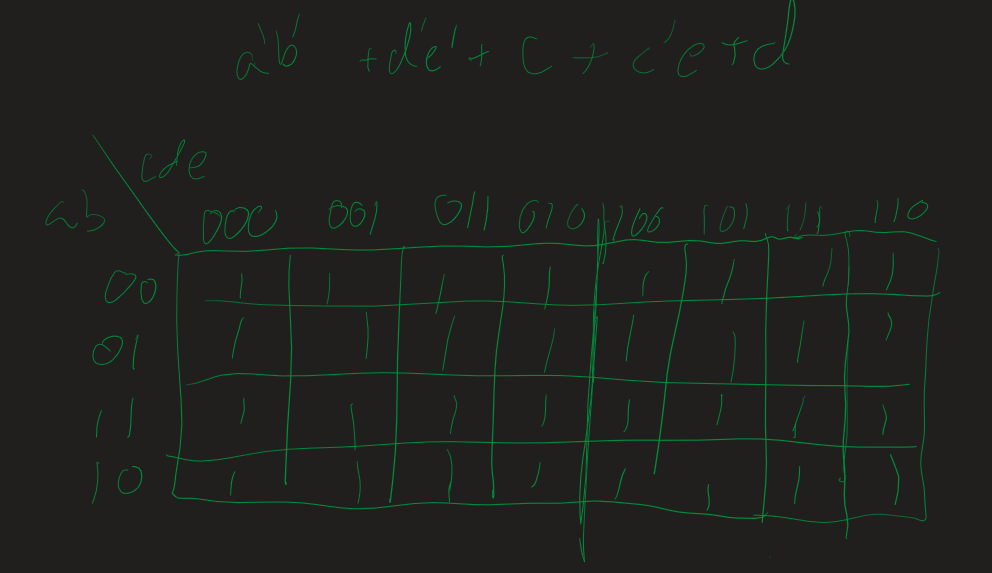
\includegraphics[width=0.95\columnwidth]{kmap_unate.png}
%  \caption{A Karnaugh map of a unate problem}\label{fig:kmap_unate}
%\end{figure}
%
%\begin{figure}
%  \centering
%  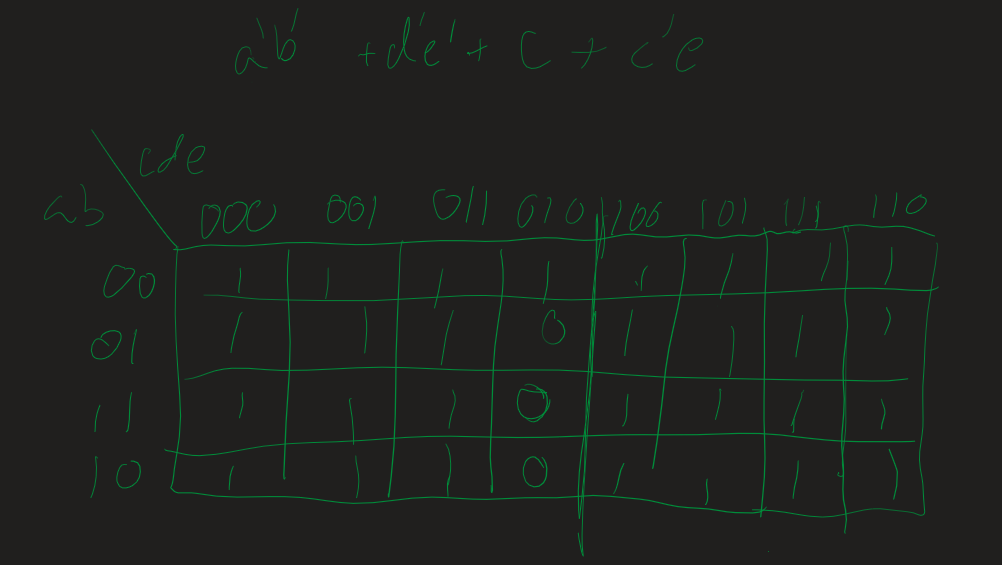
\includegraphics[width=0.95\columnwidth]{kmap_non_unate.png}
%  \caption{A Karnaugh map of a non-unate problem}\label{fig:kmap_non_unate}
%\end{figure}


%\lstinputlisting[caption=Unate output, label=lst:unate]{unate_output}
%\lstinputlisting[caption=Non-unate output, label=lst:non_unate]{non_unate_output}
%\lstinputlisting[caption=Project problem output, label=lst:example_run]{project_output}
%
%\section{Program}


\end{document}

%%% Local Variables:
%%% mode: latex
%%% TeX-master: t
%%% End:
